\documentclass[xcolor=dvipsnames,serif]{beamer}\usepackage[]{graphicx}\usepackage[]{color}
%% maxwidth is the original width if it is less than linewidth
%% otherwise use linewidth (to make sure the graphics do not exceed the margin)
\makeatletter
\def\maxwidth{ %
  \ifdim\Gin@nat@width>\linewidth
    \linewidth
  \else
    \Gin@nat@width
  \fi
}
\makeatother

\definecolor{fgcolor}{rgb}{0.345, 0.345, 0.345}
\newcommand{\hlnum}[1]{\textcolor[rgb]{0.686,0.059,0.569}{#1}}%
\newcommand{\hlstr}[1]{\textcolor[rgb]{0.192,0.494,0.8}{#1}}%
\newcommand{\hlcom}[1]{\textcolor[rgb]{0.678,0.584,0.686}{\textit{#1}}}%
\newcommand{\hlopt}[1]{\textcolor[rgb]{0,0,0}{#1}}%
\newcommand{\hlstd}[1]{\textcolor[rgb]{0.345,0.345,0.345}{#1}}%
\newcommand{\hlkwa}[1]{\textcolor[rgb]{0.161,0.373,0.58}{\textbf{#1}}}%
\newcommand{\hlkwb}[1]{\textcolor[rgb]{0.69,0.353,0.396}{#1}}%
\newcommand{\hlkwc}[1]{\textcolor[rgb]{0.333,0.667,0.333}{#1}}%
\newcommand{\hlkwd}[1]{\textcolor[rgb]{0.737,0.353,0.396}{\textbf{#1}}}%
\let\hlipl\hlkwb

\usepackage{framed}
\makeatletter
\newenvironment{kframe}{%
 \def\at@end@of@kframe{}%
 \ifinner\ifhmode%
  \def\at@end@of@kframe{\end{minipage}}%
  \begin{minipage}{\columnwidth}%
 \fi\fi%
 \def\FrameCommand##1{\hskip\@totalleftmargin \hskip-\fboxsep
 \colorbox{shadecolor}{##1}\hskip-\fboxsep
     % There is no \\@totalrightmargin, so:
     \hskip-\linewidth \hskip-\@totalleftmargin \hskip\columnwidth}%
 \MakeFramed {\advance\hsize-\width
   \@totalleftmargin\z@ \linewidth\hsize
   \@setminipage}}%
 {\par\unskip\endMakeFramed%
 \at@end@of@kframe}
\makeatother

\definecolor{shadecolor}{rgb}{.97, .97, .97}
\definecolor{messagecolor}{rgb}{0, 0, 0}
\definecolor{warningcolor}{rgb}{1, 0, 1}
\definecolor{errorcolor}{rgb}{1, 0, 0}
\newenvironment{knitrout}{}{} % an empty environment to be redefined in TeX

\usepackage{alltt}
\usetheme{Boadilla}
\usecolortheme[named=CornflowerBlue]{structure}
\usepackage{graphicx}
\usepackage{breqn}
\usepackage{xcolor}
\usepackage{booktabs}
\usepackage{verbatim}
\usepackage{tikz}
\usepackage[final]{animate}
\usepackage{lmodern}
\usetikzlibrary{shadows,arrows,positioning}
\definecolor{links}{HTML}{2A1B81}
\hypersetup{colorlinks,linkcolor=links,urlcolor=links}
\usepackage{pgfpages}

\tikzstyle{block} = [rectangle, draw, text width=9em, text centered, rounded corners, minimum height=3em, minimum width=7em, top color = white, bottom color=brown!30,  drop shadow]

% change font of frame titles and title slide
\setbeamerfont{title}{series=\bfseries}
\setbeamerfont{frametitle}{series=\bfseries} 

% enumerate style
\setbeamertemplate{enumerate items}[circle]

% my macros
\newcommand{\ShowSexpr}[1]{\texttt{{\char`\\}Sexpr\{#1\}}}
\newcommand{\Bigtxt}[1]{\textbf{\textit{#1}}}
\IfFileExists{upquote.sty}{\usepackage{upquote}}{}
\begin{document}

\title[TS decomposition]{Time series topic 2: Decomposition}

\author[M. Beck]{Marcus W. Beck\inst{1}}

\date{}

\institute[]{\inst{1} USEPA NHEERL Gulf Ecology Division\\ Email: \href{mailto:beck.marcus@epa.gov}{beck.marcus@epa.gov}}

% knitr setup


% dependents


% get online bib file


%%%%%%
\begin{frame}
\vspace{0.3in}
\centerline{
\begin{tikzpicture}
  \node[drop shadow={shadow xshift=0ex,shadow yshift=0ex},fill=white,draw] at (0,0) {
\includegraphics[width=0.9\textwidth]{imgs/workshop2016logo.png}};
\end{tikzpicture}}
\titlepage
\end{frame}

\section{Overview}

%%%%%%
\begin{frame}{Objectives for the session (3:30-4:15)}
\begin{itemize}
\item What and why time series decomposition \\~\\
\item Functions in SWMPr, other resources \\~\\
\item Application to NERRS data \\~\\
\begin{itemize}
\item Data prep \\~\\
\item Execution
\item Interpretation 
\end{itemize}
\end{itemize}
\end{frame}

%%%%%%
\begin{frame}{Interactive portion}
\onslide<+->
Follow along as we go:\\~\\
\begin{itemize}
\item flash drive\\~\\
\item online: \href{http://swmprats.net/}{swmprats.net} 2016 workshop tab \\~\\
\end{itemize}
\onslide<+->
You will run examples whenever you see this guy: \\~\\
\centerline{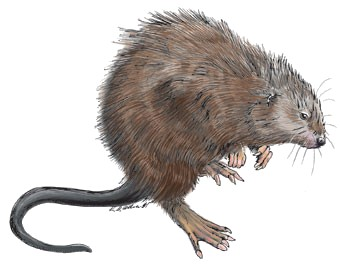
\includegraphics[width = 0.15\textwidth]{imgs/swmprat.png}} 
\end{frame}

%%%%%%
\begin{frame}[fragile]{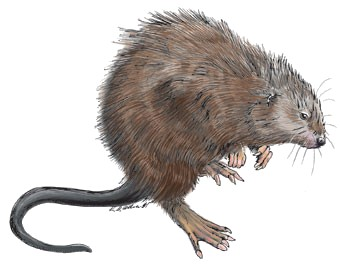
\includegraphics[width = 0.05\textwidth]{imgs/swmprat.png} Is everything installed?}
\onslide<1->
We will use functions in the SWMPr package \\~\\
Option 1, from the R Console prompt:
\begin{knitrout}\scriptsize
\definecolor{shadecolor}{rgb}{0.969, 0.969, 0.969}\color{fgcolor}\begin{kframe}
\begin{alltt}
\hlkwd{install.packages}\hlstd{(}\hlstr{'SWMPr'}\hlstd{)}
\hlkwd{library}\hlstd{(SWMPr)}
\end{alltt}
\end{kframe}
\end{knitrout}
\onslide<2->
\vspace{0.1in}
Option 2, install the source file from the flash drive:
\begin{knitrout}\scriptsize
\definecolor{shadecolor}{rgb}{0.969, 0.969, 0.969}\color{fgcolor}\begin{kframe}
\begin{alltt}
\hlcom{# change as needed}
\hlstd{path_to_file} \hlkwb{<-} \hlstr{'C:/Users/mbeck/Desktop/SWMPr-v2.1.7.9000.tar.gz'}

\hlcom{# install, load}
\hlkwd{install.packages}\hlstd{(path_to_file,} \hlkwc{repos} \hlstd{=} \hlkwa{NULL}\hlstd{,} \hlkwc{type}\hlstd{=}\hlstr{"source"}\hlstd{)}
\hlkwd{library}\hlstd{(SWMPr)}
\end{alltt}
\end{kframe}
\end{knitrout}
\end{frame}



%%%%%%
\begin{frame}[t]{Theory and background}{}
{\bf \centerline{Observed data represents effects of many processes}}
\vspace{0.15in}
\centerline{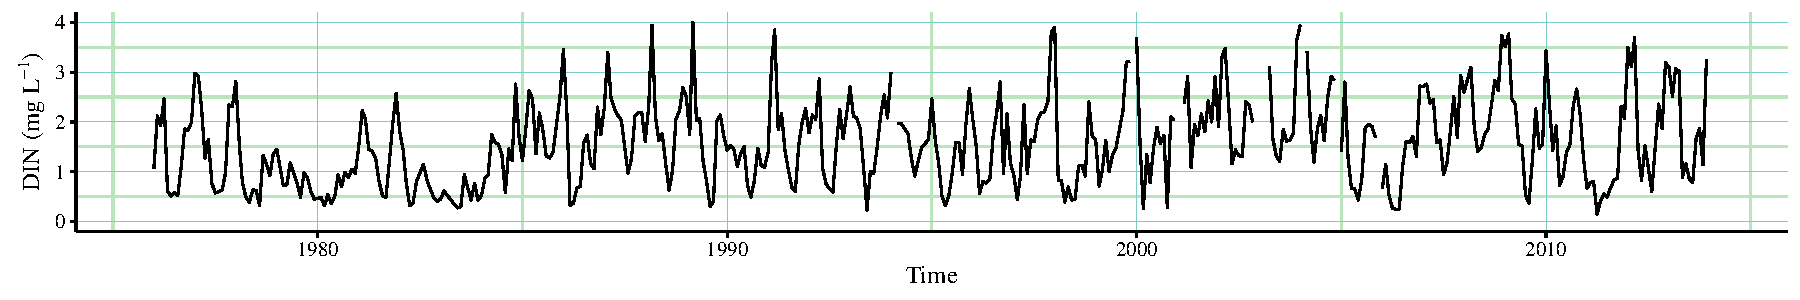
\includegraphics[width = \textwidth]{imgs/ts_ex.pdf}}
\vspace{0.15in}
\begin{columns}[t]
\begin{column}{0.3\textwidth}
{\bf \underline{\Bigtxt{Climate}}}\\
precipitation\\
temperature\\
wind events\\
ENSO effects
\end{column}
\begin{column}{0.3\textwidth}
{\bf \underline{\Bigtxt{Local}}}\\
light/turbidity\\
residence time\\
invasive species\\
trophic effects
\end{column}
\begin{column}{0.3\textwidth}
{\bf \underline{\Bigtxt{Regional/historical}}}\\
watershed inputs\\
point sources\\
management actions
flow changes
\end{column}
\end{columns}
\end{frame}

%%%%%%
\begin{frame}[t]{Theory and background}
\onslide<+->
{\bf \centerline{Observed data represents effects of many processes}}
\vspace{0.15in}
\centerline{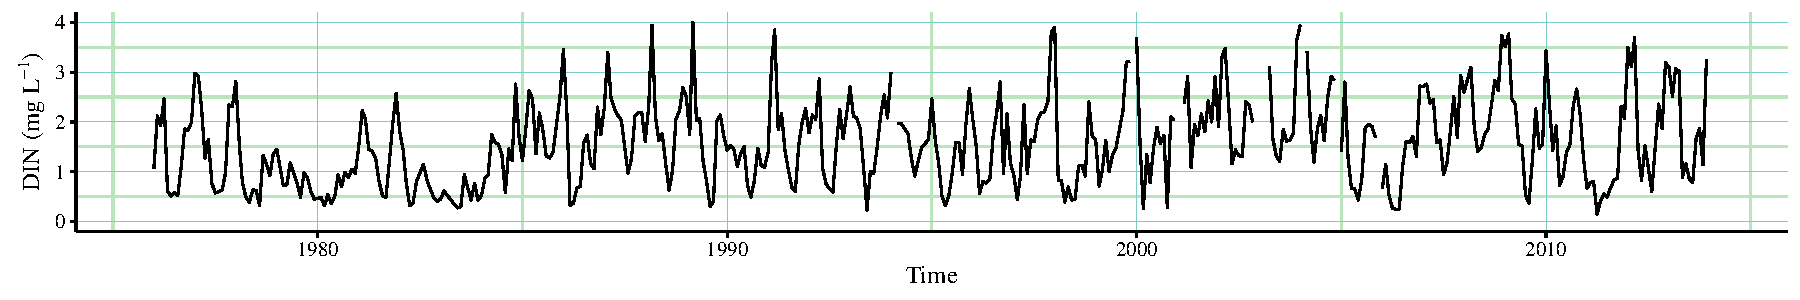
\includegraphics[width = \textwidth]{imgs/ts_ex.pdf}}
\centerline{Models should describe components to evaluate effects}
\vspace{-0.1in}
\begin{columns}[t]
\begin{column}{0.5\textwidth}
\onslide<+->{
\centerline{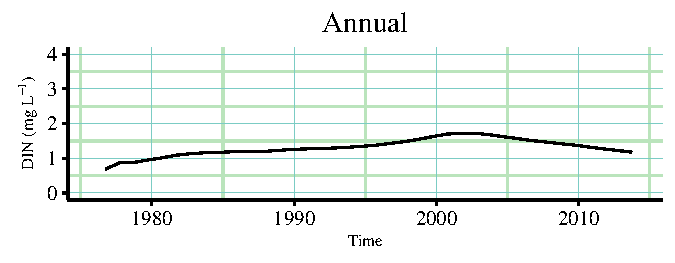
\includegraphics[width = 0.8\textwidth]{imgs/schematic2.pdf}}
\centerline{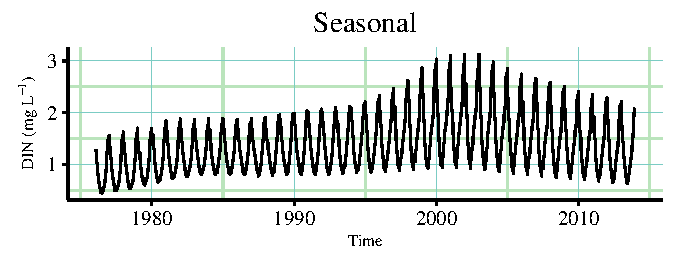
\includegraphics[width = 0.8\textwidth]{imgs/schematic3.pdf}}
}
\end{column}
\begin{column}{0.5\textwidth}
\onslide<+->{
\centerline{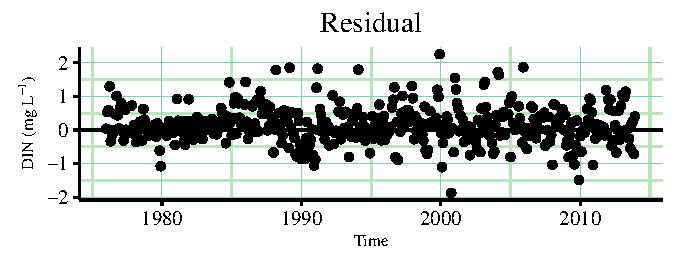
\includegraphics[width = 0.8\textwidth]{imgs/schematic4.pdf}}
\centerline{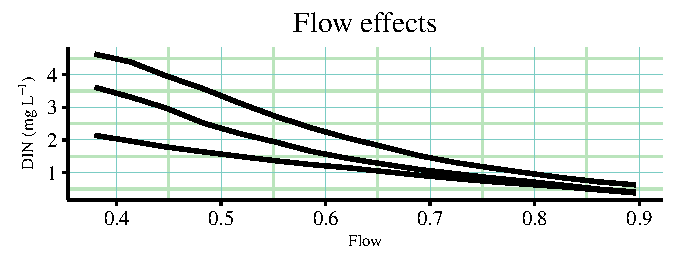
\includegraphics[width = 0.8\textwidth]{imgs/schematic5.pdf}}
}
\end{column}
\end{columns}
\end{frame}

%%%%%%
\begin{frame}{Theory and background}
\begin{itemize}
\item<1-> Time series decomposition is a very general topic - WRTDS is a form of decomposition \\~\\
\item<2-> There are more generic and simpler approaches \\~\\
\item<3-> Objective is to isolate (or remove) a \Bigtxt{known} component in a time series \\~\\
\item<4-> But be warned... just because you can doesn't mean you should
\end{itemize}
\end{frame}

%%%%%%
\begin{frame}{Theory and background}
Two very general decomposition methods are provided in SWMPr: \texttt{decomp()}, and \texttt{decomp_cj}) \\~\\
These are not new methods, they just make it easy to decompose NERRS data
\end{frame}

%%%%%%
\begin{frame}{Theory and background}

\end{frame}

\section{Application}

\section{Summary}

%%%%%%
\begin{frame}{Time series decomposition summary}{}
Things to ask before decomposition: \\~\\
\begin{itemize}
\item What is the time step? Is it regular? Does it need be standardized?
\item How do I deal with missing data?
\item Is there any expected cyclical variation? If so, what is the period (e.g., seasonal, daily)?
\item Is stationarity a reasonable expectation? 
\end{itemize}
\end{frame}

%%%%%%
\begin{frame}
\vspace{0.3in}
\centerline{
\begin{tikzpicture}
  \node[drop shadow={shadow xshift=0ex,shadow yshift=0ex},fill=white,draw] at (0,0) {
\includegraphics[width=0.9\textwidth]{imgs/workshop2016logo.png}};
\end{tikzpicture}}
\vspace{0.5in}
\centerline{Up next... Time Series Topic 3: Seasonal Kendall}
\vspace{0.5in}
\Large
\centerline{\Bigtxt{Questions??}}
\end{frame}

%%%%%%
\section{References}
\begin{frame}[t]{\textbf{References}}
\tiny
\setbeamertemplate{bibliography item}{}
\bibliographystyle{apalike_mine}
\bibliography{refs}
\end{frame}
\end{document}
